% L15a one trading day of a backtest. A time axis with three trading days, each with an open and a close.
% After the close of day t, the method computes the wealth W(t), updates the estimates, and checks the six
% triggers. With no trigger, it keeps the portfolio (gray). When a trigger fires (orange, the trigger color of
% Fig-L15a-Gamma-Picks), it makes a new decision: pick a basket, weight it, and queue the orders, which
% fill at the open of day t + 1. The gray arc shows yesterday's orders filling at the open of day t.
%
% November 26, 2026: drawn in the style of the L13a schematics (schematic-style.tex), matching the backtest
% algorithm of the lecture (run_study in code/src/mpc/StudyBacktest.jl: fill at the open, compute the wealth at the close,
% check the triggers, decide, and queue the orders for the next open).
\documentclass[tikz,border=6pt]{standalone}
% Shared style for the L15a schematics, copied from L14a (November 19, 2026), \input by each Fig-L15a-*.tex.
% Copied from week-13/L13a/figs/jumphmm-diagram.tex (the week-12 schematic style): same fonts,
% ink, accent colors, boxes, and arrows, plus a monospace font for tool names and order
% statuses. The notebook SVG carries a dark palette added by theme_svg.py; every color here
% must be mapped there.
\usepackage[no-math]{fontspec}
\IfFontExistsTF{Arial}{\setsansfont{Arial}}{\setsansfont{TeX Gyre Heros}}
\renewcommand{\familydefault}{\sfdefault}
\IfFontExistsTF{Menlo}{\setmonofont[Scale=0.92]{Menlo}}{}
\usepackage{amsmath,amssymb}
\usetikzlibrary{arrows.meta,calc,positioning,decorations.pathreplacing}

\definecolor{vnink}{HTML}{202124}
\definecolor{gdblue}{HTML}{0091FF}
\definecolor{gdred}{HTML}{E02020}
\definecolor{gdgray}{HTML}{6D7278}
\definecolor{saorange}{HTML}{F08C00}
\definecolor{boxfill}{HTML}{F1F3F4}
\definecolor{orangefill}{HTML}{FFE8C7}
\definecolor{bluefill}{HTML}{E5F3FF}
\definecolor{redfill}{HTML}{FDE8E8}
\definecolor{gridgray}{HTML}{E3E5E8}

\tikzset{
  every picture/.append style={x=1cm, y=1cm, font=\sffamily\small, text=vnink},
  % boxes and arrows, as in the L12a schematics
  flow/.style={draw=vnink, line width=0.9pt, -{Latex[length=2.4mm, width=1.7mm]}},
  feedback/.style={draw=saorange, line width=1.2pt, -{Latex[length=2.6mm, width=1.9mm]}, rounded corners=6pt},
  sumbox/.style={draw=vnink, fill=boxfill, line width=0.8pt, rounded corners=3pt, inner sep=5pt, align=center},
  note/.style={text=gdgray, font=\sffamily\footnotesize, align=center},
  state/.style={circle, draw=vnink, fill=white, line width=1.0pt, minimum size=1.1cm, inner sep=0pt, font=\sffamily\normalsize},
  % plots, as in the L10b profit diagrams
  axis/.style={draw=vnink, line width=0.8pt, -{Latex[length=2.6mm, width=1.8mm]}},
  spine/.style={draw=vnink, line width=0.8pt},
  curve/.style={draw=vnink, line width=1.6pt, line join=round, line cap=round},
  series/.style={draw=gdgray, line width=0.9pt, line join=round},
  drop/.style={draw=gdgray, line width=0.8pt, dash pattern=on 3pt off 2pt},
  pt/.style={circle, draw=vnink, fill=white, line width=1.0pt, inner sep=0pt, minimum size=2.0mm},
}


\begin{document}
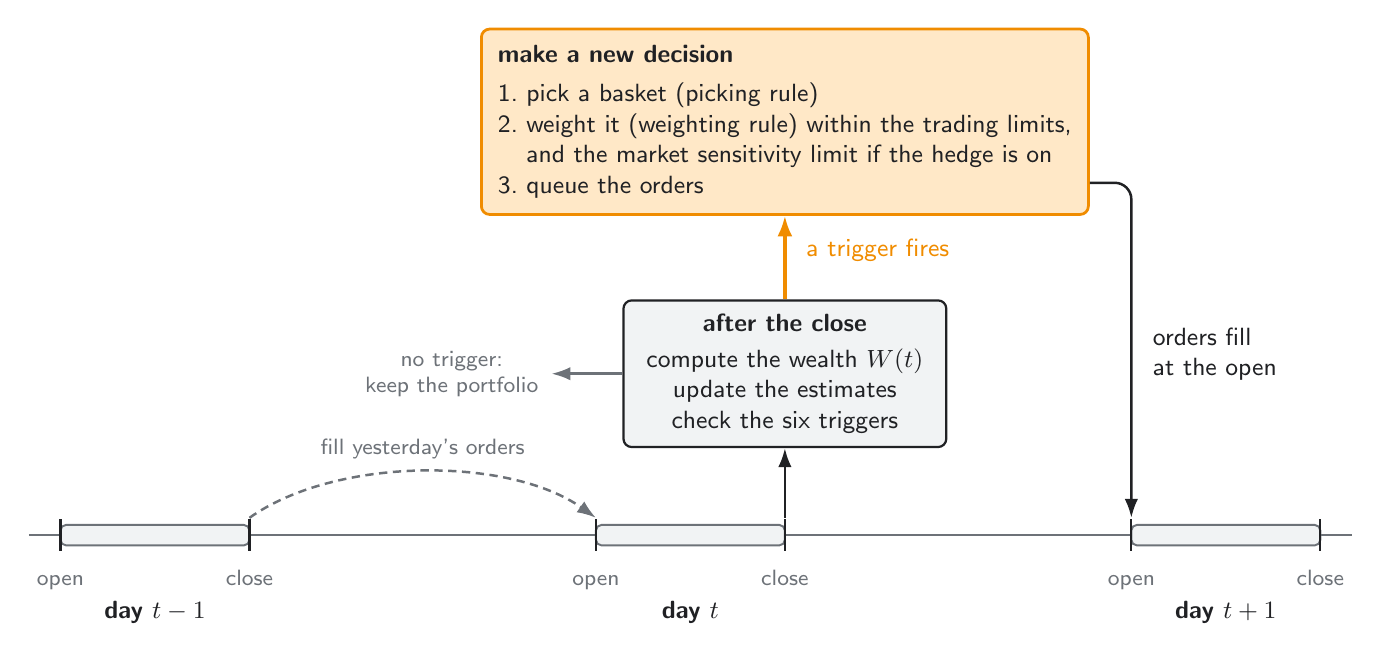
\begin{tikzpicture}[
  session/.style={draw=gdgray, fill=boxfill, line width=0.7pt, rounded corners=2pt},
  back/.style={draw=gdgray, line width=0.9pt, -{Latex[length=2.4mm, width=1.7mm]}},
  decision/.style={draw=saorange, fill=orangefill, line width=1.0pt, rounded corners=3pt, inner sep=6pt, align=left},
]
  % ---------------------------------------------------------------- three trading days
  \draw[spine, draw=gdgray] (-0.4, 0) -- (16.4, 0);
  \foreach \o/\c/\name in {0.0/2.4/{day $t-1$}, 6.8/9.2/{day $t$}, 13.6/16.0/{day $t+1$}} {
    \draw[session] (\o, -0.13) rectangle (\c, 0.13);
    \draw[spine] (\o, -0.2) -- (\o, 0.2);
    \draw[spine] (\c, -0.2) -- (\c, 0.2);
    \node[note, anchor=north, text height=1.6ex, text depth=0.3ex] at (\o, -0.27) {open};
    \node[note, anchor=north, text height=1.6ex, text depth=0.3ex] at (\c, -0.27) {close};
    \node[font=\sffamily\small\bfseries, anchor=north] at ({(\o + \c)/2}, -0.72) {\name};
  }

  % ---------------------------------------------------------------- after the close of day t
  \node[sumbox, align=center, minimum width=4.1cm] (close) at (9.2, 2.05)
    {\textbf{after the close}\\[2pt] compute the wealth $W(t)$\\ update the estimates\\ check the six triggers};
  \draw[flow] (9.2, 0.22) -- (close.south);

  % no trigger: keep the portfolio
  \draw[back] (close.west) -- ++(-0.9, 0) node[note, anchor=east, xshift=-1pt] {no trigger:\\keep the portfolio};

  % a trigger fires: a new decision
  \node[decision] (decide) at (9.2, 5.25)
    {\textbf{make a new decision}\\[3pt]
     1.\ pick a basket (picking rule)\\
     2.\ weight it (weighting rule) within the trading limits,\\
     \phantom{2.\ }and the market sensitivity limit if the hedge is on\\
     3.\ queue the orders};
  \draw[feedback] (close.north) -- (decide.south);
  \node[font=\sffamily\small, text=saorange, anchor=west] at (9.35, 3.62) {a trigger fires};

  % the orders fill at the next open
  \coordinate (queue) at ($(decide.south east) + (0, 0.42)$); % the level of step 3, queue the orders
  \draw[flow, rounded corners=6pt] (queue) -- (13.6, 0 |- queue) -- (13.6, 0.22);
  \node[font=\sffamily\small, anchor=west, align=left] at (13.75, 2.3) {orders fill\\at the open};

  % the orders of the day before fill at the open of day t
  \draw[back, dash pattern=on 3pt off 2pt] (2.4, 0.22) .. controls (3.5, 1.0) and (5.7, 1.0) .. (6.8, 0.22);
  \node[note, anchor=south] at (4.6, 0.84) {fill yesterday's orders};
\end{tikzpicture}
\end{document}
